\documentclass[12pt]{article}
\usepackage[a4paper]{geometry}
\usepackage{fullpage}
\usepackage[T1]{fontenc}
\usepackage[utf8]{inputenc}
\usepackage{graphicx}
\usepackage{mathpazo}
\pagenumbering{gobble}
\usepackage{siunitx}
\sisetup{output-decimal-marker = {,}}
\usepackage{amsmath}
\usepackage{esdiff}
\usepackage[spanish]{babel}
\usepackage{cancel}
\newcommand{\laplace}[1]{\mathbf{#1}(\mathbf{s})}
\newcommand{\slp}{\mathbf{s}}

\begin{document}

\title{\textsc{Teoría de Circuitos III}\\Prueba BT5 (Turno 1)}

\date{21 de enero de  2019\\\small{Los resultados se publicarán el 22 de enero.\\La revisión del examen se realizará los días \textbf{23 y 24} de enero de 2019 de \textbf{11:30 a 13:30}.}}

\maketitle

El circuito de la figura representa una fuente de corriente alterna sinusoidal alimentando un cuadripolo $Q_1$ que, a su vez, está conectado a una impedancia de carga. 
\begin{enumerate}
\item Determina los parámetros impedancia del cuadripolo.
\item A partir del resultado obtenido en el apartado anterior, calcula la impedancia de entrada del cuadripolo. A partir de este resultado, obtén la impedancia que debe tener el generador para se produzca máxima transferencia de potencia.
\item Determina los parámetros admitancia de un cuadripolo, $Q_T$, conformado por una asociación paralelo-paralelo de dos cuadripolos $Q_1$ idénticos. Dibuja los circuitos necesarios para comprobar si existe interacción entre los cuadripolos (test de Brune), y razona el resultado que se obtendría en este caso. 
\item ¿Cuál es la impedancia de entrada del cuadripolo $Q_T$ si en su puerto de salida tiene la misma impedancia $\overline{Z}_L$?
\end{enumerate}


\begin{minipage}{0.3\textwidth}
  Datos:
  \begin{itemize}
  \item $R$ = \SI{1}{\ohm}
  \item $X_C$ = \SI{2}{\ohm}
  \item $\overline{Z}_L$ = -j\SI{2}{\ohm}
  \end{itemize}
\end{minipage}
\begin{minipage}{0.7\textwidth}
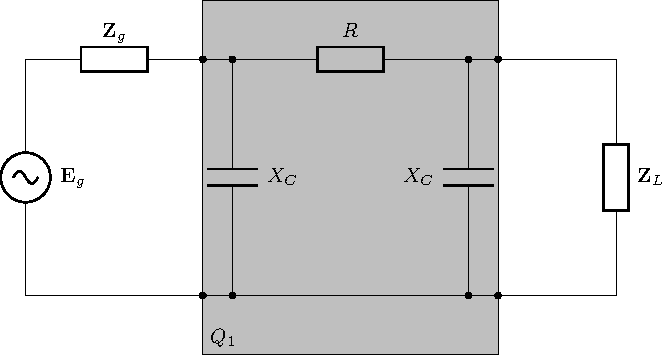
\includegraphics{figs/E5_circuito.pdf}
\end{minipage}

\vspace*{1cm}

\clearpage

\subsection*{Solución}

\begin{enumerate}
\item Parámetros impedancia

  Para obtener los parámetros impedancia se pueden aplicar directamente las ecuaciones de esta familia. Otra opción es obtener los parámetros admitancia, dado que se trata de un circuito $\pi$, y transformar a parámetros impedancia. En cualquier caso, el resultado es:

\[
  [\overline{Z}] = 
  \left[
    \begin{array}{cc}
      0.235 - 1.059j & -0.235 - 0.941\\
      -0.235-0.941j & 0.235 - 1.059j\\
    \end{array}
  \right]
\]

Comprobamos que la matriz cumple las propiedades de un circuito recíproco y simétrico.

\item Impedancia de entrada.

  Teniendo en cuenta las ecuaciones de los parámetros impedancia, y con la ecuación del puerto de salida obtenemos la expresión de la impedancia de entrada al cuadripolo:

  \[
    \overline{Z}_i = \overline{Z}_{11} - \frac{\overline{Z}_{12} \overline{Z}_{21}}{\overline{Z}_L + \overline{Z}_{22}}
  \]

  Sustituyendo valores obtenemos:

  \[
    \overline{Z}_i = \SI[parse-numbers=false]{0.4 - 0.8j}{\ohm}
  \]

  Por tanto, para que se produzca máxima transferencia de potencia, la impedancia del generador debe ser:

  \[
    \overline{Z}_g = \overline{Z}_i^* = \SI[parse-numbers=false]{0.4 + 0.8j}{\ohm}
  \]
  
\item Asociación paralelo-paralelo

  Este circuito cumple el test de Brune por su propia construcción. Por tanto,

  \[
    [\overline{Y}_T] = 2 \cdot [\overline{Y}] =
      \left[
    \begin{array}{cc}
      2 + j & -2\\
      -2 & 2 + j\\
    \end{array}
  \right]
  \]
donde los parámetros admitancia se han obtenido invirtiendo la matriz de impedancias del primer apartado.
\item Impedancia de entrada de la asociación
  Con el resultado anterior obtenemos la matriz de parámetros impedancia del cuadripolo $Q_T$.
  \[
    [\overline{Z}_T] = 
      \left[
    \begin{array}{cc}
      -0.118 - 0.529j & -0.118 - 0471j\\
      -0.118 - 0.471j & -0.118 - 0.529j\\
    \end{array}
  \right]
  \]

  Utilizando la expresión anterior para la impedancia de entrada obtenemos ahora:

  \[
    \overline{Z}_{iT} = \SI[parse-numbers=false]{0.165 - 0.449j}{\ohm}
  \]
  
\end{enumerate}

\end{document}

% Local Variables:
% ispell-local-dictionary: "castellano"
% End:

